\documentclass[letterpaper, 12pt]{report}
\usepackage[utf8]{inputenc}
\usepackage[english, spanish]{babel}
\usepackage{fullpage} % changes the margin
\usepackage{graphicx} 
\usepackage{enumitem} 
\usepackage{chngcntr}
\usepackage{setspace}
\counterwithin{figure}{section}
\renewcommand{\thesection}{\arabic{section}} 
\renewcommand{\thesubsection}{\thesection.\arabic{subsection}}
\renewcommand{\baselinestretch}{1.5}
\usepackage{float}
\bibliographystyle{apalike}
\setlength\belowcaptionskip{10pt}
\linespread{1.5}

\begin{document}

\begin{titlepage}
	\centering
	
\includegraphics[width=0.3\textwidth]{Images/logo_utb.png}\par\vspace{1cm}
	{\scshape\LARGE Universidad Tecnológica de Bolívar \par}
	\vspace{1cm}

	{\scshape\Large FÍSICA ELÉCTRICA \par}
	\vspace{.2cm}

	% chktex-file 8
	{\scshape\Large H1 - C \par}
	\vspace{1cm}
	% chktex-file 8
	\slshape {\Large \bfseries{} LAB 3 - SUPERFICIES EQUIPOTENCIALES Y LÍNEAS
		DE CAMPO ELÉCTRICO  \\}
	\vspace{1cm}

	\slshape {\itshape{} Mauro González, T00067622 \\}
	\slshape {\itshape{} German De Armas Castaño, T00068765 \\}
	\slshape {\itshape{} Angel Vega Rodriguez, T00068186 \\}
	\slshape {\itshape{} Juan Jose Osorio Ariza, T00067316 \\}
	\slshape {\itshape{} Juan Eduardo barón, T00065901 \\}
	\vfill
	Revisado Por \\
	Gabriel Hoyos Gomez Casseres\\
	{\large \today\par}
\end{titlepage}

% ----------------------------------------------------------------------|>
\section{Introducción}

En el siguiente pre informe se abordaran temáticas necesarias para  explicar
las características y comportamiento del potencial eléctrico, variando las
distancias a una carga fuente y variando la magnitud de la carga con el fin
de establecer resultados y conclusiones precisas sobre su dirección, 
geometría y distribución.

\vspace{.5cm}

Además, se busca entender los conceptos relacionados a la practica que puedan 
resultar en factores determinantes como lo puede ser el mismo campo eléctrico 
en sí, porque dependiendo de cómo se altere o manipule tendría una consecuencia 
directa con el resultado del experimento a realizar, modificando en gran 
medida su representación.

\newpage

% ----------------------------------------------------------------------|>
\section{Objetivos}

\subsection{Objetivos Generales}

\begin{itemize}
	\item Dibujar lineas de campo eléctrico
	\item Analizar las diferentes características equipotenciales y también
	      las lineas de campo eléctrico.
	\item Comprender la relación que existe entre potencial eléctrico y
	      campo eléctrico
\end{itemize}

\newpage

% ----------------------------------------------------------------------|>
\section{Preparación de la practica}

% -------------------------------------|>
\subsection{¿Qué son superficies equipotenciales?}
Las superficies equipotenciales son aquellas en las que el potencial toma un
valor constante.

Por ejemplo, las superficies equipotenciales creadas por
cargas puntuales son esferas concéntricas centradas en la carga, como se
deduce de la definición de potencial.\hfill\break{}~\cite{blas_fernández}

% -------------------------------------|>
\subsection{¿Cómo se calcula el campo eléctrico estático en un punto del espacio a partir del valor del
	potencial en ese punto?}

La relación entre campo eléctrico y el potencial es:

$\int_{a}^{b} E \cdot\,dl \longrightarrow$ Va - Vb

~\cite{PotencialElectrico}

% -------------------------------------|>
\subsection{¿Por qué las líneas de campo eléctrico que pasan por una superficie equipotencial deben ser
	perpendiculares a la superficie?}

Tomando como referencia una esfera con carga equitativamente distribuida,
la simetría de la distribución esférica hace que para puntos exteriores a
la esfera se comporte como si toda la carga se encontrara concentrada en
el centro de la esfera, por lo que las líneas de campo deberán ser radiales
y, al ser la carga positiva, dirigidas hacia fuera de la carga.

\vspace{.5cm}

Las superficies equipotenciales deberán ser superficies esféricas concéntricas
decreciendo los potenciales hacia el exterior.

\vspace{.5cm}

En el caso de la placa plana cargada negativamente, las consideraciones sobre
la simetría nos llevan a asegurar que las líneas de campo llevarán la
dirección perpendicular a la placa y el sentido hacia la misma. Además
deberán estar uniformemente distribuidas como resultado de que el campo se
mantiene constante mientras nos alejamos de las mismas. Por tanto las
superficies equipotenciales serán planos paralelos a la placa y haciéndose
mayores conforme nos alejamos de la placa (menos negativos al alejarnos).
~\cite{LineasCampoElectrico}

% -------------------------------------|>
\subsection{Lineas de campo eléctrico}

\begin{figure}[H]
	\begin{center}
		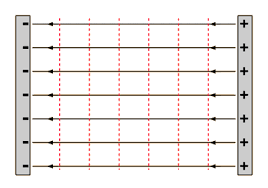
\includegraphics[scale = 1]{./Images/A.png}
		\caption{(A) Electrodos Paralelos}
	\end{center}
\end{figure}

\begin{figure}[H]
	\begin{center}
		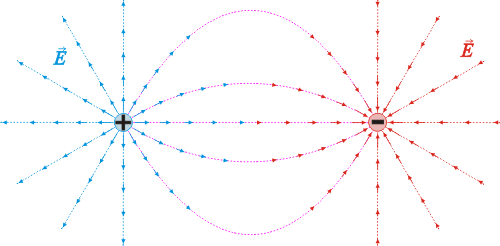
\includegraphics[scale = .8]{./Images/B.png}
		\caption{(B) Electrodos puntuales de diferente signo}
	\end{center}
\end{figure}

\begin{figure}[H]
	\begin{center}
		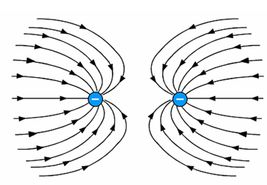
\includegraphics[scale = 1]{./Images/C.png}
		\caption{(C) Electrodos puntuales de igual signo}
	\end{center}
\end{figure}

\begin{figure}[H]
	\begin{center}
		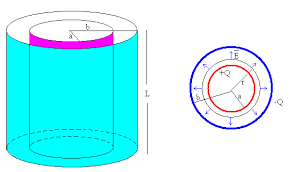
\includegraphics[scale = 1.4]{./Images/D.png}
		\caption{(D) Electrodos concéntricos}
	\end{center}
\end{figure}

% ----------------------------------------------------------------------|>
\section{Resumen del procedimiento}

\begin{itemize}
	\item Ajustar un voltaje de 10V en el panel de fuentes teniendo en cuenta
	      que debe estar en la salida D.C.
	\item Se procede a armar el montaje colocando en distintas posiciones el
	      polo positivo y el negativo para poder establecer un sistema de
	      coordenadas cartesianas sobre el papel.
	\item Seleccione un punto que tengan la misma diferencia de potencial con
	      al electrodo negativo e ir registrando los valores con sus respectivas
	      coordenadas.
	\item Luego desplace  la sonda positiva y seleccione otro punto que al
	      medir la diferencia de potencial sea igual a la del punto anterior y
	      repetirlo hasta que cubra la región entre los electrodos y que tengan las
	      mismas distancias entre estos.
	\item Por último, repetir todo el procedimiento para encontrar más grupos
	      de puntos con igual diferencia de potencia.
\end{itemize}


\newpage
\bibliography{./Bibliography/bibliography.bib}

\end{document}